\section{Terrain following advection of a stable thermal profile}
\label{sec:wobblyThetaAdvection}

This test is designed to confirm that the potential temperature errors found in the gravity waves test are due to advection.  The same potential temperature profile from the gravity waves test is advected over BTF and SnapCol grids using a terrain following velocity field that imitates a physical flow over orography.

\subsection{Specification}
The spatial domain, mountain profile and potential temperature profile are the same as those from the gravity waves test.  The potential temperature profile is fixed at the inlet and zero gradient at the outlet boundary so that it is advected consistently.  The upwind-biased advection scheme is used, as described in section~\ref{sec:method:discretisation}.  Following the gravity waves test, the model is integrated forward by 5 hours with a timestep $\Delta t = \SI{8}{\second}$. 

The velocity field is given by equation~\ref{eqn:wobblyTracerAdvection:velocity} but, because the mountain profile is different, the derivative of terrain height, $\partial h / \partial z$, is
\begin{align}
\frac{\partial h}{\partial x} &= - 2 h_0 \exp \left( - \left( \frac{x}{a} \right)^2 \right) \cos \left( \frac{\pi x}{\lambda} \right) \left[
\frac{\pi}{\lambda} \sin \left(\frac{\pi x}{\lambda} \right) +
\frac{x}{a^2} \cos \left( \frac{\pi x}{\lambda} \right) \right]
\end{align}

\subsection{Results}

\TODO{l2 error norm?}
\TODO{sample line, as with gravityWaves?}

\begin{figure}
	\captionsetup[subfigure]{position=b}
	\centering
	\subcaptionbox{BTF \label{fig:wobblyThetaAdvection:thetaDiff:btf}}[0.49\textwidth]{\includegraphics[height=2.6in,angle=270]{openfoam/cases/wobblyThetaAdvection/btf/schaerExp/cubicUpwindCPCFit/18000/thetaDiff.eps}}
	\hfill
	\subcaptionbox{SnapCol \label{fig:wobblyThetaAdvection:thetaDiff:snapCol}}[0.49\textwidth]{\includegraphics[height=2.6in,angle=270]{openfoam/cases/wobblyThetaAdvection/snapCol/schaerExp/cubicUpwindCPCFit/18000/thetaDiff.eps}}
%
	\caption{Potential temperature anomalies of terrain following advection of a stable potential temperature profile at $t = \SI{18000}{\second}$. \TODO{colour legend}}
	\label{fig:wobblyThetaAdvection:thetaDiff}
\end{figure}
